\subsection{Damping}
\begin{frame}
\tableofcontents[currentsection]
\end{frame}

\begin{frame}
\frametitle{Algoritmo implementato}
\begin{center}
Abbiamo adoperato un'oppurtuna normalizzazione del termine forzante poich\'e non usiamo variabili scalate (ordine del drogaggio)
\begin{equation*}
\begin{array}{l}
F_k = F(\varphi_k) \quad F_{k+1}=F(\varphi_k+t_k^{(j)}\delta\varphi_k) 
 \\  
t_k^{(j)}=\frac{1}{1+K_k^{(j)}\parallel F_k\parallel}  
\quad \longrightarrow \quad \parallel F_k\parallel \approx 10^{18}\Longrightarrow t_k^{(j)} \approx 0
\\  
N\approx 10^{18} \quad \tilde{t}_k^{(j)}=\frac{1}{1+K_k^{(j)}\parallel F_k\parallel_\infty N^{-1}}  
\\ 
K_k^{(j)} \quad t.c. \quad
1-\frac{\parallel F_{k+1}^{(j)} \parallel_\infty}{  \parallel F_{k} \parallel_\infty }< \delta \tilde{t}_k^{(j)} \quad\quad K_k^{(j)} = K_{base}^j
\end{array}
\end{equation*}
\begin{alertblock}{Problema}
La condizione di uscita non viene mai soddisfatta, si esce dal ciclo solo perch\`e viene opportunamente settato il maxit su $j$ (altrimenti $t_k^{(j)}\rightarrow 0$ e il sistema non evolve).
\end{alertblock}
\end{center}
\end{frame}

\begin{frame}
\frametitle{Andamento del residuo}
Comportamenti differenti del residuo sulla risoluzione di Newton senza damping al variare dei drogaggi.
\begin{center}
\begin{figure}[!h]
          {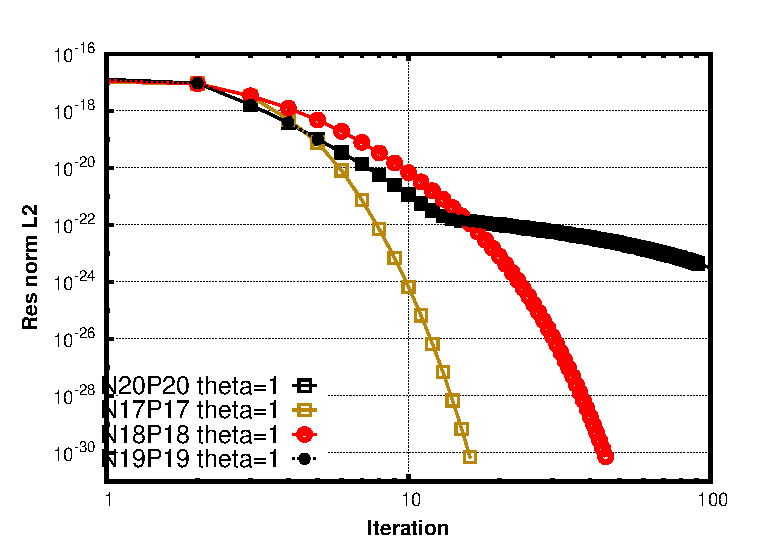
\includegraphics[scale=0.6]{Cfr_Doping}}

\end{figure}
\end{center}


\end{frame}

\begin{frame}
\frametitle{Damping}
\begin{columns}
\begin{column}{0.5 \textwidth}
\begin{exampleblock}{Parametri settati da input file}
\begin{itemize}
\item[-] $K_{base}$
\item[-] $\delta$
\item[-] N (fattore di normalizzazione)
\end{itemize}
\end{exampleblock}
\end{column}
\begin{column}{0.4 \textwidth}
$NOTA:$ abbiamo usato il caso N20P20 pi\`u lento a convergere
\end{column}
\end{columns}
\begin{center}
\begin{figure}[!h]
          {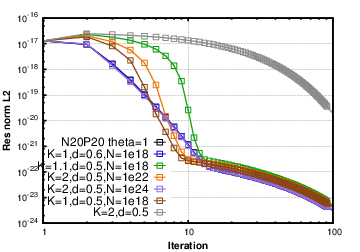
\includegraphics[scale=0.58]{Cfr_DAMPING}}
\end{figure}
\end{center}
\end{frame}


